\documentclass{article}

\usepackage[utf8]{inputenc}
\usepackage{amsmath}
\usepackage{amsfonts}
\usepackage{amssymb}
\usepackage{graphicx}
\usepackage[table,xcdraw]{xcolor}
\usepackage[hidelinks]{hyperref}
\usepackage{fontawesome5}


\graphicspath{ {./images/} }

\renewcommand{\contentsname}{Indice}

\makeatletter
\newcommand*{\rom}[1]{\expandafter\@slowromancap\romannumeral #1@}
\makeatother

\usepackage[a4paper,top=2cm,bottom=2cm,left=2cm,right=2cm]{geometry}


\title{\textbf{\Huge Specifica dei Requisiti}}
\author{Edoardo Ghirardello, Giulio Cappelli, Elia Casotti \\ \\ Gruppo T42}
\date{2022}

\let\origthesubsection\thesubsection

\begin{document}

\maketitle

\clearpage
\tableofcontents
\clearpage

\section{Scopo del documento}
\begin{description}
    \item[] Questo documento riporta la specifica dei requisiti di sistema del sistema "Fen Festa", impiegando diversi tipologie di diagrammi UML quali:
        \begin{itemize}
            \item Diagramma dei Casi d'Uso (Use-Case Diagram)
            \item Diagramma di Contesto (Context Diagram)
            \item Diagramma dei Componenti (Component Diagram)
        \end{itemize}
\end{description}
\clearpage
\section{Requisiti Funzionali}
\begin{description}
    \item[] Nel seguente capitolo vengono riportati i Requisiti Funzionali (RF) del sistema utilizzando il linguaggio naturale e Use Case Diagram scritti in UML
\end{description}
\renewcommand\thesubsection{RF\arabic{subsection}}
\subsection{Visualizzazione eventi}
\subsection{Ricerca Eventi}
\subsection{Visualizzazione descrizione evento (Utente Non Registrato)}
\subsection{Visualizzazione descrizione evento (Utente Registrato)}
\begin{center}
    \item[] 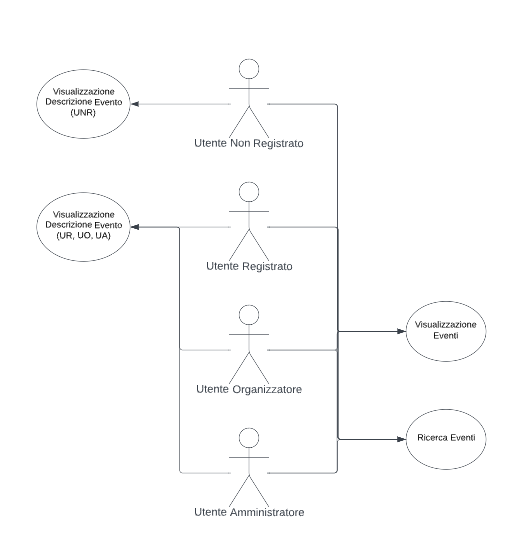
\includegraphics[scale=0.7]{UseCase_1.png}
\end{center}
\subsubsection*{Descrizione Use Case "Visualizzazione eventi"}
\begin{description}
    \item[] Titolo: Visualizzazione Evento
    \item[] Riassunto: Questo Use Case descrive come avviene la visualizzazione di un evento
    \item[] Descrizione:
        \begin{enumerate}
            \item L'utente UNR, UR, UO o UA accedono alla pagina "Home" dove visualizzeranno la lista degli eventi
            \item L'utente sceglie il range temporale in cui filtrare gli eventi (Giorno, Settimana, Mese) tramite un selezionatore di data
            \item Il sistema poi mostrerà tutti gli eventi aventi la data o il range temporale selezionato
        \end{enumerate}
        % \item[] Exceptions:
        %     \begin{description}
        %         \item[] [exception 1]
        %     \end{description}
        % \item[] Extensions:
        %     \begin{description}
        %         \item[] [extension 1]
        %     \end{description}
\end{description}
\renewcommand\thesubsection{\origthesubsection}
\clearpage
\section{Requisiti Non Funzionali}
\begin{description}
    \item[]
\end{description}
\clearpage
\section{Analisi del Contesto}
\begin{description}
    \item[]
\end{description}
\clearpage
\section{Analisi dei Componenti}
\begin{description}
    \item[]
\end{description}
\end{document}